% Author: Bhishan Poudel
% Date  : Mar 2, 2018
% Update:
%
%
%#*******************************************************
%#=======================================================
%# Chapter 5: Shear Analysis
%#=======================================================
%#*******************************************************
%
%
\section{Chapter 5: Shear Analysis}\label{sec:chap5}
From the galaxy simulation program \textbf{Jedisim}, we get monochromatic and chromatic LSST simulated galaxies. We intend to
analyze the shear of these galaxies. For the shear analysis I use a program called \textbf{imcat}\footnote{https://www.ifa.hawaii.edu/~kaiser/imcat/}. First we create the parameter file for the psf called 'psf.par'. Then we create the lc catalog files for all of the chromatic and monochromatic files. From 1000 simulations files of chromatic and monochromatic files we get 1000 catalog files. We combine them and do some galaxy cutting, for example: 'rg > 2.9' and so on. After that we use the imcat command `etprofile` to get the ellipticities and shears. For the simulations we used redshift z = 0.7, F814W filter HST images. The results are given below:
\begin{figure}[ht!]
    \centering
    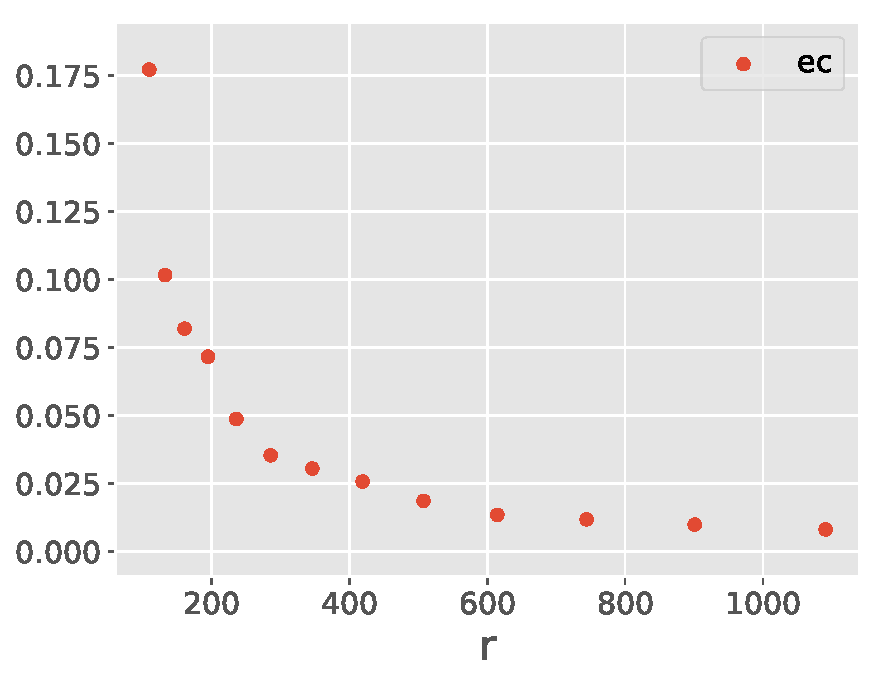
\includegraphics[width=0.48\textwidth,height=0.6\textwidth]{ec}
    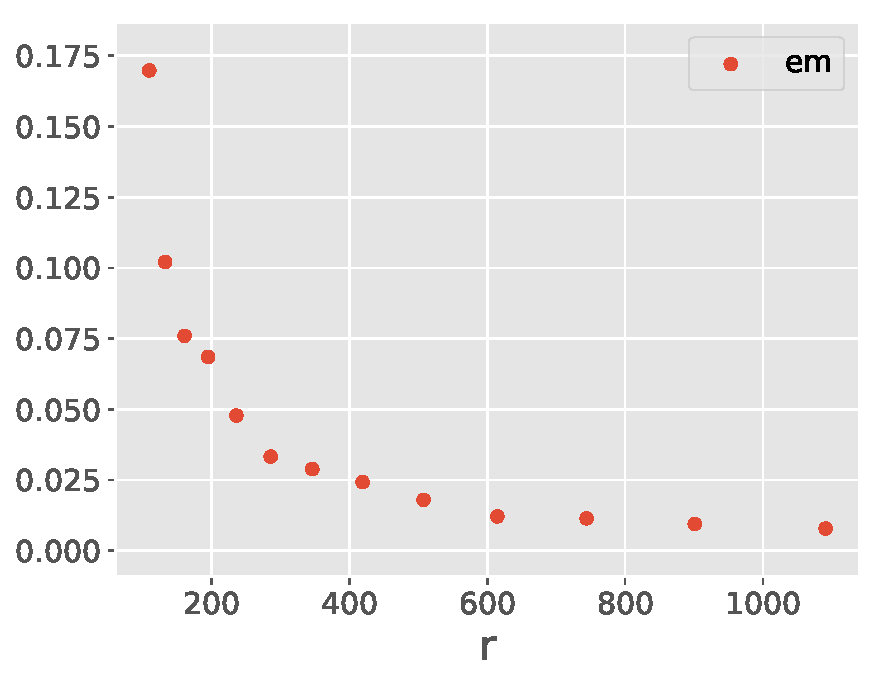
\includegraphics[width=0.48\textwidth,height=0.6\textwidth]{em}
    \caption{Ellipticites for chromatic and monochromatic files}
\end{figure}

\newpage
\begin{figure}[ht!]
    \centering
    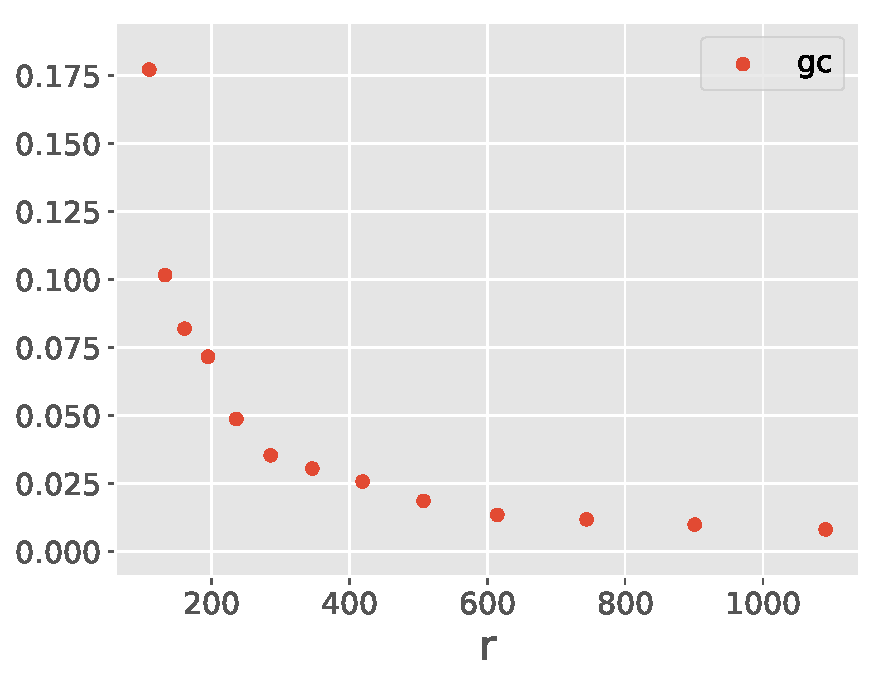
\includegraphics[width=0.48\textwidth,height=0.5\textwidth]{gc}
    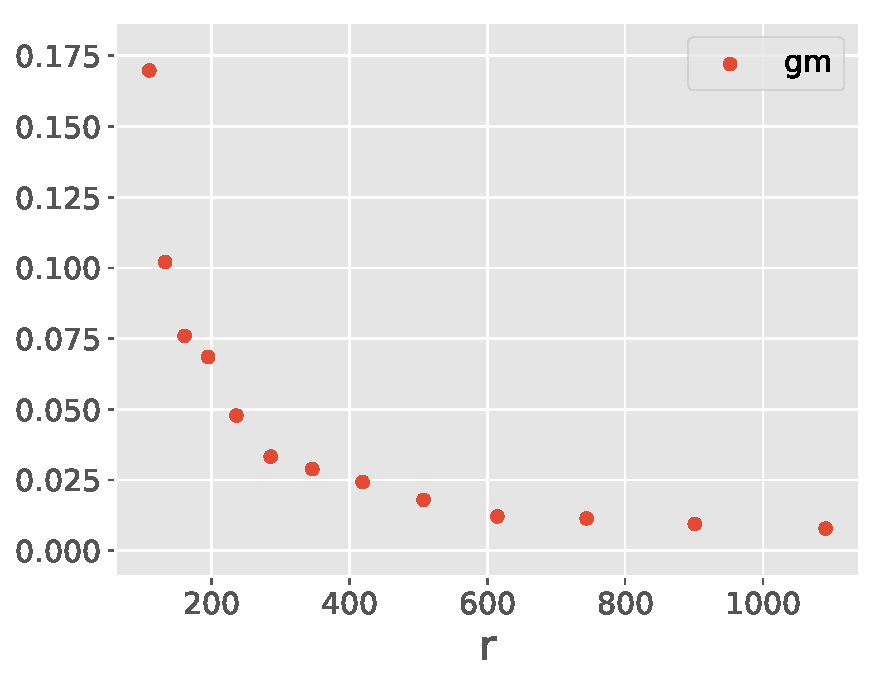
\includegraphics[width=0.48\textwidth,height=0.5\textwidth]{gm}
    \caption{Shears for chromatic and monochromatic files}
\end{figure}

\begin{figure}[ht!]
    \centering
    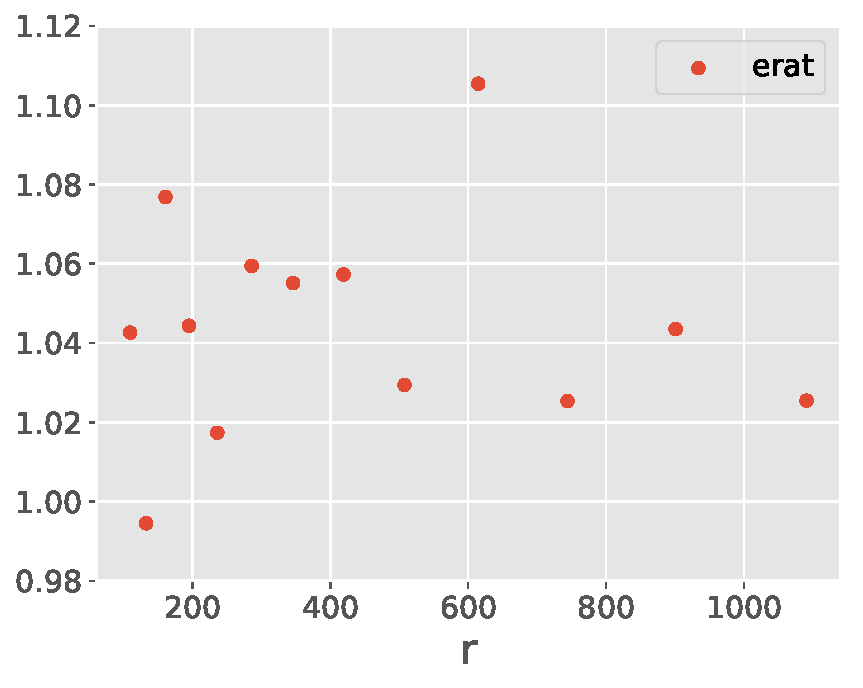
\includegraphics[width=0.48\textwidth,height=0.5\textwidth]{erat}
    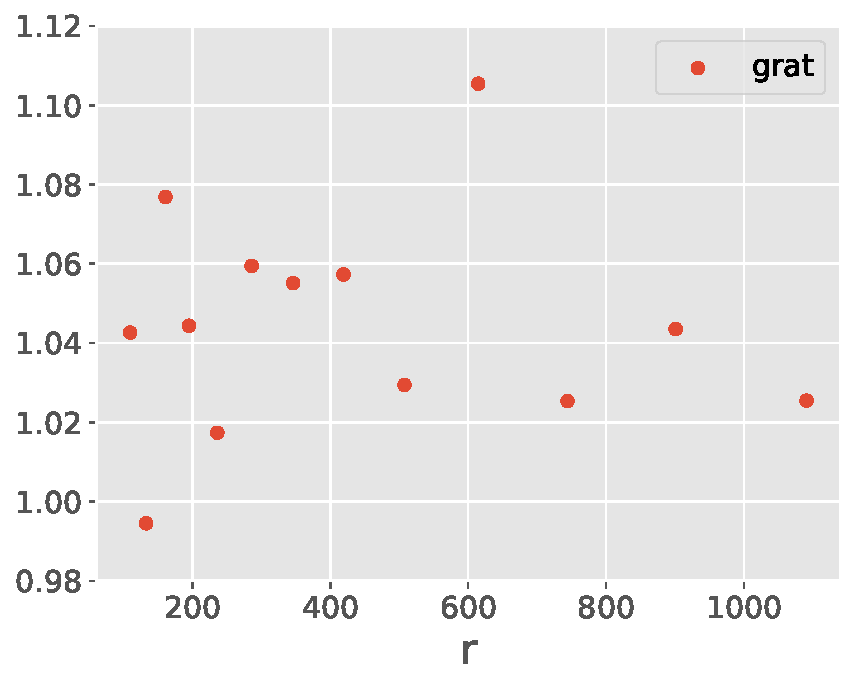
\includegraphics[width=0.48\textwidth,height=0.5\textwidth]{grat}
    \caption{Ellipticites and Shears Ratio (chromatic/monochromatic) }
\end{figure}